\documentclass{beamer}
\newif\ifplacelogo
\placelogotrue
\mode<presentation>{\usetheme{Boadilla2}}

\usepackage{geometry}
\usepackage{color}
\usepackage{graphicx}

\usepackage[T1]{fontenc}
\usepackage{fontspec}
\setmainfont{CenturyGothic}
\setsansfont{CenturyGothic}

\AtBeginSection[]{\frame{\tableofcontents[currentsection]}}

\definecolor{myturquoise}{RGB}{0,176,176}
\definecolor{mylightturquoise}{RGB}{54,216,216}


\begin{document}


\setlength{\unitlength}{1mm}
\title{DS Visualisation and Analysis}
\author[Abbey Waldron]{Abbey Waldron}
\date[September 18th, 2015]{}




\setbeamertemplate{navigation symbols}{}

{
\placelogofalse
\begin{frame}
  \titlepage
\end{frame}
}



\begin{frame}{This Week - Correlations and Functional Forms}

\begin{enumerate}
\item Show last week's work to the class
\item What is a correlation?
\item Some maths\ldots describing (functional) relationships
\item Start work on problems
\end{enumerate}

\end{frame}



\begin{frame}{Random Student Generator}

\end{frame}


\begin{frame}{Week 2 Problems: West Africa Ebola}

Make one plot to answer each question.

\begin{enumerate}
\item Which country has the most rapid initial rise in ebola cases?
\item How does the total number of ebola deaths change over time?
\item When do new country infections occur?
\item What are the per country confirmed case totals per month in 2014?
\item Make one more plot to show something interesting.
\end{enumerate}



\end{frame}


\begin{frame}{Continuing your R education\ldots}

Sometimes the easiest way to perform these tasks is with looping:
\begin{itemize}
\item http://blog.datacamp.com/tutorial-on-loops-in-r/
\end{itemize}

\end{frame}


\begin{frame}{Correlation}
\end{frame}

\begin{frame}{Correlation}

Strong/Weak?

\vspace{5mm}

Direction?

\vspace{5mm}

Linear/Non-linear\ldots?

\end{frame}


\begin{frame}{Correlation}

\begin{center}
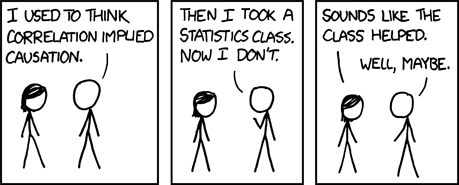
\includegraphics[scale=0.7]{pics/wk3/correlation.png}
\end{center}

xkcd.com/552


\end{frame}


\begin{frame}{Causation}

CORRELATION DOES NOT IMPLY CAUSATION

\end{frame}



\begin{frame}{Causation?}

\begin{center}
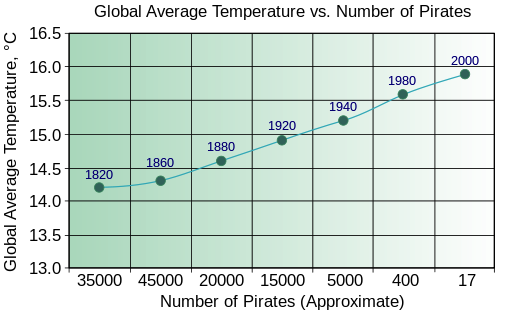
\includegraphics[scale=0.6]{pics/wk3/pirates_new.png}
\end{center}

(Thank you Wikipedia!)


\end{frame}


\begin{frame}{Causation?}
\vspace{-5cm}
\begin{center}
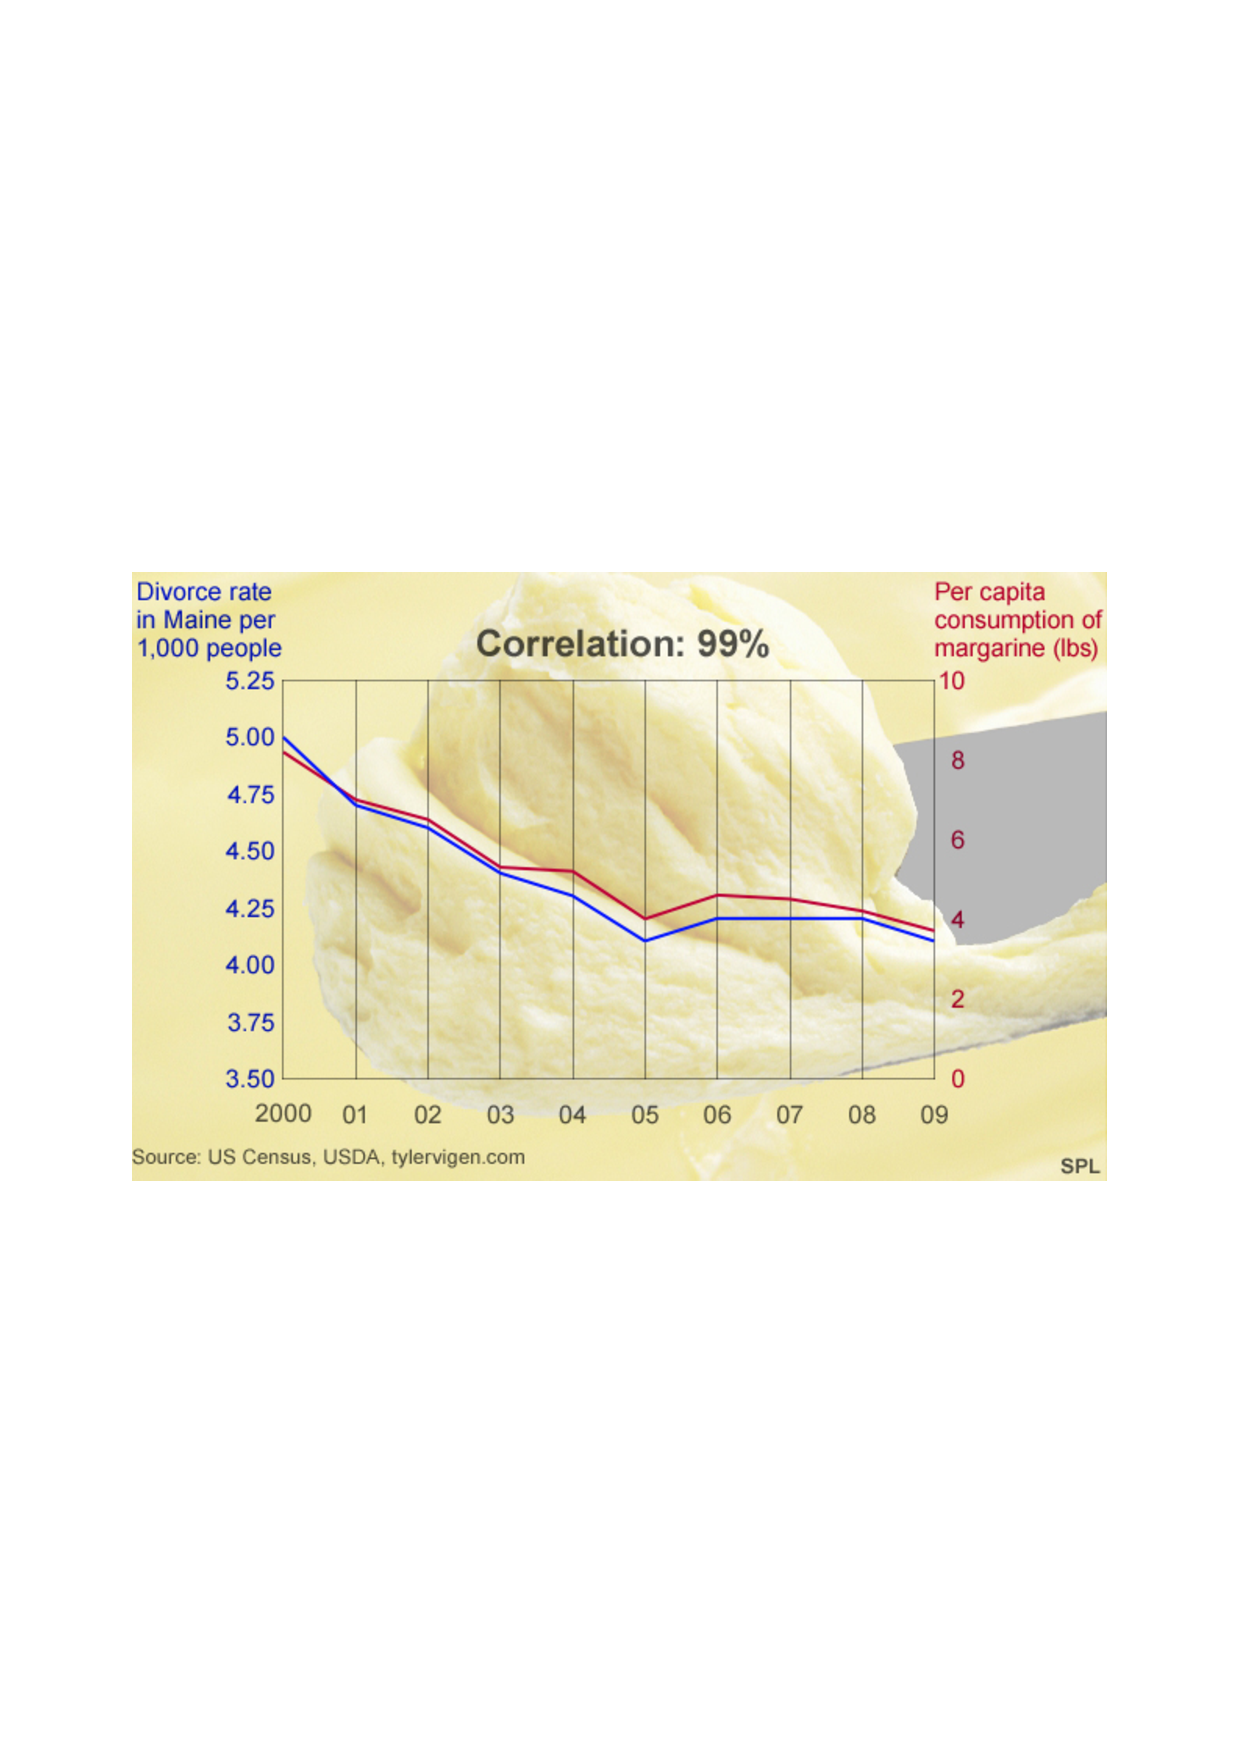
\includegraphics[scale=0.6]{pics/wk3/marg.pdf}
\end{center}


\end{frame}



\begin{frame}{Types of Causation}

If A and B are correlated then there are different possibilities of causation:
\begin{itemize}
\item A causes B
\item B causes A
\item C causes A and B (lurking factor)
\item A causes C which causes B (or vice versa)
\item A causes B and B causes A (cyclic or bidirectional)
\item there is no connection between A and B only coincidence
\end{itemize}


\end{frame}





\begin{frame}{How to discover correlations?}

\end{frame}


\begin{frame}{How to discover correlations?}

Make some plots!!  Of course\ldots

\begin{itemize}
\item Typically make scatterplots of each pair of variables
\item Can you see a relationship?  If not then not strong.
\item Describe relationships using functions (not only linear!)
\end{itemize}

\end{frame}


\begin{frame}{R makes this easy\ldots}

Look at \texttt{pairs()}

\end{frame}



\begin{frame}{Functions}

\end{frame}



\begin{frame}{Functions}

In general, plot the dependent values on the y (vertical) axis and the independent values on the x (horizontal) axis, but the difference is not always there.

\begin{displaymath}
y = f(x) = ...
\end{displaymath}

\end{frame}


\begin{frame}{Function Examples}


\begin{itemize}
\item linear, quadratic, cubic\ldots polynomial
\item exponential, logarithmic
\item Gaussian
\item etc.
\end{itemize}


\end{frame}



\begin{frame}{Why we need to be quantative\ldots}

Later on we are going to try to use some variables to predict others, this requires fitting a sensible function to the available data.

\vspace{5mm}

These problems come in two main categories:
\begin{enumerate}
\item You have a theoretical model for how the variables should be related
\item You have no theoretical model for the relationship and you have to guess somehting from the data
\item Some combination of the two due to \textit{e.~g.~}unexpected noise.
\end{enumerate}

\end{frame}



\begin{frame}{The second case: guessing functions}

Often there is not a single right answer (theme of this course\ldots)

\vspace{5mm}

Which function is good enough?
\begin{itemize}
\item Needs to describe the major features of the data
\item Should be minimal - as simple as will work
\item May well not be unique, you can try fitting different functional forms and see which one works best
\item We will start the actual fitting next week
\end{itemize}


\end{frame}


\begin{frame}{What is a feature?}


Things to look for and check match:
\begin{itemize}
\item behaviour as $x \rightarrow \pm \infty$
\item turning points (gradient = 0)
\item crossing points with the axes
\end{itemize}

\end{frame}



\begin{frame}{Week 3 Problems}

\begin{enumerate}
\item Finding and describing correlations
\item Functional forms
\end{enumerate}



\end{frame}




%%%%%%%%%%%%% backup slides %%%%%%%%%%%%%%%%%%%%%%%%

\appendix
\newcounter{finalframe}
\setcounter{finalframe}{\value{framenumber}}

\begin{frame}{Backup Slides}
\end{frame}




\setcounter{framenumber}{\value{finalframe}}

\end{document}
